\chapter{绪论}
\label{chap:introduction}

\section{论文研究背景及应用}
\label{s:background}
信息隐藏技术是信息安全领域中一个重要的研究方向,它是一种将数据嵌入到各种载体中的
技术,它被大量应用在隐秘通信、篡改认证和版权保护中。狭义的信息隐藏技术,被称为隐
写术(Steganography)。隐写术将秘密消息隐藏在一些公开传输的媒介中,利用公开媒介
来掩护消息的传输,主要关注通信的隐蔽性。隐写术要求对载体进行微量的随机修改,以防
止被隐藏的消息被通信对端以外的第三方发现。与隐写术相对的技术称为隐写分析技术
(Steganalysis)。它通过对公开传输媒介的统计特征进行分析,以判断媒介中是否被隐藏
了消息。对隐写、隐写分析的研究有助于对非法活动进行监控,对维护社会稳定,保护国家
及人民安全有着至关重要的作用。
\par
但是隐写术并不关心对载体的保护,当秘密消息被提取后,载体通常不能被完美地恢复。而
这种情况在一些应用中是不允许的,例如以医疗、军事图像为载体的信息隐藏,这些应用对
图像质量有着相当高的要求,即使微小的改变也不能被接受。因此,学者们提出了可逆的信
息隐藏(Reversible Data Hiding,RDH)技术。可逆信息隐藏技术不仅关注秘密消息,同
时也关注对载体本身的保护。通过特殊的嵌入算法,载体的原始信息被保护起来,当消息被
提取之后,原始信息能够被可逆的恢复。同隐写不同的是,大多数可逆隐藏算法并不关注
消息本身的隐蔽性,它不被用来进行隐蔽通信。
\par
由于可逆隐藏技术载体可恢复的特点,它在现实生活中得到了广泛的应用,具体应用如下:
\par
%\vspace{-2mm}
\begin{itemize}
  \setlength{\parindent}{2em}
  \vspace{-3mm}
  \item \textbf{信息管理}
  \vspace{-2mm}
  \par
  随着互联网的发展,网络上的数据量日益增大,如何对如此庞大的数据进行管理是一个
  关键的问题。文献\cite{hwang2010trusted}中,作者基于可逆信息隐藏,提出了一种
  云计算的保障机制。作者在云端服务器存储的用户数据中嵌入了对应的用户信息,节省
  了大量的数据库空间。另外,在医院,常常将患者的个人隐私信息通过可逆隐藏技术
  嵌入到医学图像当中,这样既可以起到隐私保护的目的,又可以对大量图像进行管理。
  \par
  \vspace{-3mm}
  \item \textbf{完整性认证}
  \vspace{-2mm}
  \par
  PS、Audition等数字媒体处理软件的出现使得网络上出现了众多虚假的照片、音频,使
  人难辨真伪。而利用信息隐藏,可以在载体中嵌入与载体高度相关的哈希特征值,或者
  载体的参考信息(Reference Value)。这样当使用者得到这些载体时,他们可以重新
  计算载体哈希特征,与其中嵌入的特征进行比较,以判断载体是否被修改,以及在什么
  位置被修改,甚至利用参考信息,恢复出原始载体的部分或全部信息。而由于信息嵌入
  的可逆性,当载体没有被破坏时,原始载体可以被完美恢复。
  \par
  \vspace{-3mm}
  \item \textbf{版权信息保护}
  \vspace{-2mm}
  \par
  被用于版权信息保护的信息隐藏技术通常又被称为数字水印(Digital Watermarking)
  技术或者数字指纹技术(Digital Fingerprint)。水印技术通过将商业产品标识,如
  特征码,商标等信息嵌入到产品中,指示产品的版权归属。而数字指纹技术则常常将
  已授权用户的相关信息嵌入到产品当中,通过检测盗版产品中的用户相关信息就可以
  追查到盗版源头。这种技术同人类指纹有着相似的作用,因此被称为数字指纹,以防
  止合法用户未经许可散播产品给未授权用户。\\
\end{itemize}



\section{可逆信息隐藏技术的分类}
\label{s:type_application_reversible_data_hiding}
\begin{figure}[!ht]
\centering 
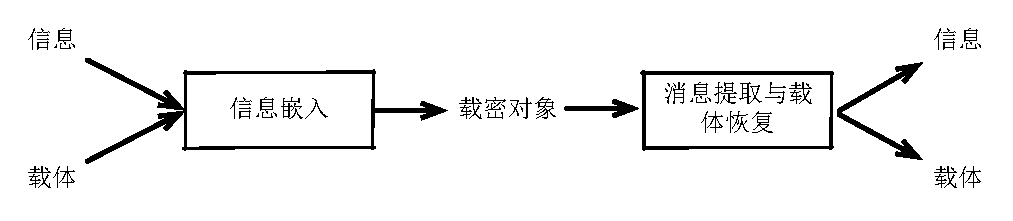
\includegraphics[width=0.7\textwidth]{figures/reversible_framework.eps}
\caption{可逆信息隐藏的一般框架}
\label{fig:revers_framework}
\end{figure}
自从可逆隐藏技术提出以来,这个领域的研究就非常的活跃,学者们提出了各种各样有效
的算法。图\ref{fig:revers_framework}是可逆信息隐藏系统的一般框架,基本所有的算
法有符合这个框架。在``信息嵌入''模块,秘密信息被嵌入载体对象中,得到载密对象。接
收方利用``信息提取与载体恢复''算法,从载密对象中提取出秘密信息,并恢复出原始载体。
一般认为,信息嵌入过程不能对载体对象造成明显的修改。现有的可逆隐藏算法根据它们
的载体、稳健性等方面的差异,可以分为不同的类型。\\
\vspace{-8mm}
\begin{itemize}
  \setlength{\parindent}{2em}
  \vspace{-2.5mm}
  \item \textbf{以载体类型分类}\\
  \vspace{-10mm}
  \begin{itemize}
    \setlength{\parindent}{2em}
    \item[*] \textbf{基于空域图像}
    \vspace{-1mm}
    \par
    基于空域图像的可逆隐藏算法得到了广泛的研究,大多数算法都以8比特灰度图像为载
    体,对像素进行一定的修改,以达到可逆隐藏的目的。本质来说,针对空域图像的可逆
    隐藏算法同可逆压缩算法类似,都需要找到像素间的相关性,通过可逆手法去除
    像素相关以腾出空间嵌入秘密信息。不同的算法在不同的嵌入率下有着不同的表现,有
    的算法针对小嵌入率进行特殊的改进,以最大限度的提高图像质量;有的算法则注重嵌
    入容量,期望在可以容忍的图像质量下尽可能提高嵌入率。
    \par
    \vspace{-2mm}
    \item[*] \textbf{基于JPEG图像}
    \vspace{-1mm}
    \par
    JPEG作为当今最为流行的图像压缩算法,在可逆隐藏中也同样得到了深入关注。JPEG压
    缩基于DCT变换,而针对JPEG图像的可逆压缩算法也主要集中在对DCT变换系数,量化表
    等方面。本质上,DCT变换也是一种去除图像块冗余的算法,因此JPEG图像天然地使用
    于做可逆隐藏。一种常见的算法是利用每个图像块DCT系数中的0系数,例如可以寻找特
    殊的全零模式,因此这样的每个‘0’模式都可以被用来嵌入1比特信息。
    \par
    \vspace{-2mm}
    \item[*] \textbf{基于其他载体}
    \vspace{-1mm}
    \par
    随着可逆隐藏技术的不断发展,学者们不在将眼光局限在图像领域,他们尝试将可逆隐
    藏算法应用到更广泛的载体中。例如一些一维信号如音频、心电图。还有一些文献则将
    可逆隐藏的思想应用到了视频领域\cite{xu2014improved},提出了针对H.264视频的视
    频容错编码方法。文献将可逆隐藏技术同冗余片进行结合,能很有效的保障移动通信中
    的视频质量。\\
  \end{itemize}
  \vspace{-11mm}
  \item \textbf{以稳健性分类}\\
  \vspace{-10mm}
  \begin{itemize}
    \setlength{\parindent}{2em}
    \item[*] \textbf{脆弱水印}
    \vspace{-1mm}
    \par
    所谓脆弱水印,是一种当载体遭到修改后很容易被改变或毁掉的印记。由此可见,脆弱
    水印并不适合进行版权保护等工作,因为攻击者很容易就可以破坏载体中的水印。然而
    正是脆弱水印的这种对修改的敏感性,使得其被广泛的应用于图像鉴别、图像完整性认
    证等应用中。而同签名技术相比,脆弱水印被嵌入到了载体中而不需要任何的附加信息,
    节省了通信成本。另一方面,脆弱水印能够更加精确地定位篡改位置,从而使得重传成
    本进一步降低。
    \par
    \vspace{-2mm}
    \item[*] \textbf{稳健水印}
    \vspace{-1mm}
    \par
    同脆弱水印对修改的敏感性不同,稳健水印要求载体中的水印信息在载体遭到一定的攻
    击(如压缩、加噪、滤波)时,仍然不能收到破坏,能够被提取出来完成认证工作。稳
    健水印的这种特性可以被用来进行版权认证等工作。另外,稳健水印的一些特性可以用
    在隐写等隐蔽通信的应用中。例如利用一些水印的抗打印、抗拍照等特性,可以将秘密
    信息隐藏到照片中,利用照片传递来进行秘密通信。\\
  \end{itemize}
\end{itemize}



\section{本文研究内容及论文结构}
\label{s:contribution_of_this_thesis}
如前所述,当前信息隐藏研究重点主要集中在灰度图像上,不论是狭义上的隐写技术,还
是可逆隐藏技术,针对灰度图像的算法在过去得到了广泛的研究。然而在现实生活中,使
用最多的却是彩色图像,针对彩色图像的可逆隐藏算法将是未来的研究热点。
\par
同灰度图像不同,彩色图像有R、G、B三个通道,这三个通道间存在着高度的相关性,这些
相关性为可逆隐藏提供了良好的条件。本论文中提出了一种简单的基于彩色图像通道相关性
的可逆隐藏算法。论文中发现,当通过通道内的预测去除通道内相关性之后,三个通道的预
测误差的大小和结构基本相同。据此,论文提出了采用通道间进行二阶预测的算法。另外,
论文使用了一种新的排序算法:利用像素的邻域像素对预测误差的分布参数进行预测。利用
论文提出的算法,彩色图像的可逆隐藏算法的嵌入容量和图像质量得到了一定程度的提升。
\par
本论文一共分为四章,各章的内容如下:
\par
第一章主要介绍论文的研究背景,简单介绍了信息隐藏技术,对可逆隐藏技术进行了分类,
并简单介绍了隐写技术、可逆信息隐藏技术的分类和应用,简单陈述了论文的主要内容和
论文结构。
\par
第二章对主流的针对灰度空域图像的常用可逆隐藏算法,以及算法中常用的排序技术进行
了详细的介绍,算法包括基于可逆隐藏的算法,基于直方图平移、差值扩展、预测误差扩
展的算法,基于整数变换的算法等,最后则介绍了一种最新的针对彩色图像的可逆隐藏算
法。
\par
第三章则详细介绍分析了本论文提出的基于彩色图像通道相关性的算法。本章主要从预测
算法、排序算法、完整的嵌入算法及流程图以及实验结果四个角度对算法进行详细的展示。
\par
第四章将对本文的工作做出一定的总结,分析现有工作的不足之处,并对可能的后续工作
进行了展望。\\
